\chapter{Funktionsweise der Komponenten}\label{ch:funktionsweise_der_komponenten}
Die folgenden Abschnitte beschreiben die Funktionsweise der Mustererkennung in Vuforia und bieten einen grundlegenden Überblick über den Aufbau einer Unity-Anwendung.
\section{Mustererkennung in Vuforia}\label{mustererkennung_vuforia}
Vuforia ist ein Augmented Reality Software Development Kit für die Erstellung von Augmented Reality (AR) Anwendungen auf mobilen Geräten und Tablets.
Verschiedene Ziele können in Echtzeit erkannt und verfolgt werden, was die Möglichkeit bietet, virtuelle Objekte wie 3D Modelle in Bezug auf diese Ziele in der realen Welt zu positionieren.
Das virtuelle Objekt verfolgt dann die Position und Ausrichtung des Bildes in Echtzeit, sodass die Perspektive des Betrachters erhalten und das virtuelle Objekt als ein Teil der realen Szene erscheint.
Das Vuforia SDK unterstützt eine Vielzahl von 2D- und 3D-Zieltypen, einschließlich „markerloser“ Bildziele und eine Form von adressierbaren Referenzmarken, die als \textquote{VuMark} bezeichnet werden (vgl \cite{Vuforia2018}). 

Für das beschriebene IT Projekt war die performante Nutzung von zweidimensionalen Bildzielen ausreichend, da nur auf dem Globus angebrachte Markierungen erkannt werden mussten.

Vuforia bietet über eine Schnittstelle zur Unity Game Engine sowohl die Möglichkeit der nativen AR-Entwicklung für iOS und Android, als auch die Möglichkeit der Entwicklung von AR-Anwendungen in Unity, die anschließend auf beide Plattformen portierbar sind.

Das Architekturmodell \ref{fig:vuforia_architektur} beschreibt die Funktionsweise des Vuforia SDKs im Zusammenspiel mit der Unity Engine. Die Abbildung ist angelehnt auf das Vuforia-Architekturmodell in cite{MECS2015} und wurde in Hinblick auf die für das IT Projekt relevanten Aspekte vereinfacht.

\begin{figure} [h]
\centering
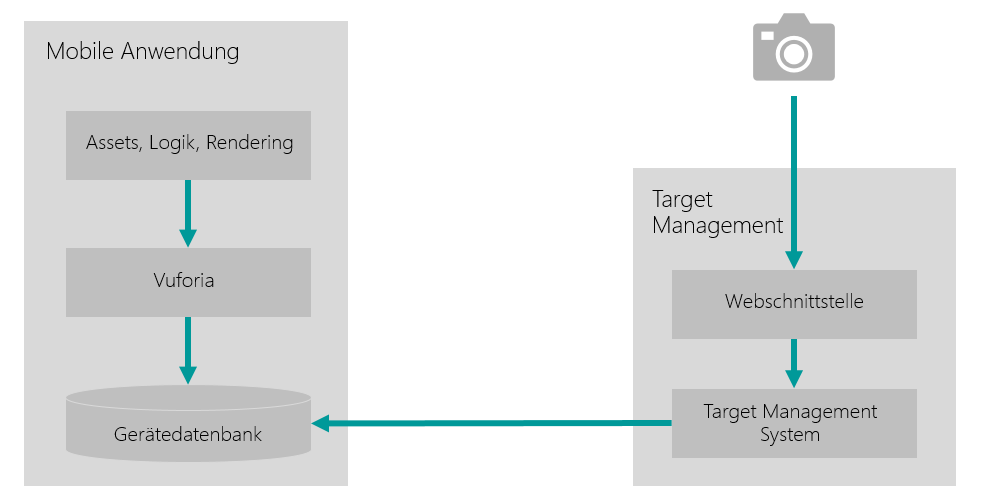
\includegraphics[width=14cm]{vuforia_architektur.PNG}
\caption{Funktionsweise von Vuforia}
\label{fig:vuforia_architektur}
\end{figure}
 
Um Bildziele für die spätere Verwendung in Unity zu generieren, muss der Benutzer selbstgewählte Bilder über die Weboberfläche des \textquote{Target Management Systems} in das System laden.
Bei der Erstellung eines solchen Image Targets ist die Angabe eines Bildnamens und einer Referenzgröße erforderlich, welche sich an der tatsächlichen Größe der verwendeten Marker orientiert.
Das Target Management System liefert dem Nutzer eine Bewertung der erwarteten Erkennungs- und Verfolgungsleistung des Ziels, sowie eine Visualisierung der von der Vuforia Engine verwendeten Merkmale des Ziels, beispielhaft dargestellt in Abbildung \ref{fig:image_target_rating}. 
Diese Erkennungsmerkmale sind die im Muster gelb eingefärbten Stellen.
Um ein hohes Rating und somit eine gute Bilderkennung zu gewährleisten, sollte deshalb auf die Wahl von geeigneten Image Targets geachtet werden.
Die Kriterien bei dieser Auswahl, sowie die Integration der fertigen Image Targets werden in Abschnitt \ref{einbindung_mustererkennung} beschrieben.

\begin{figure} [h]
\centering
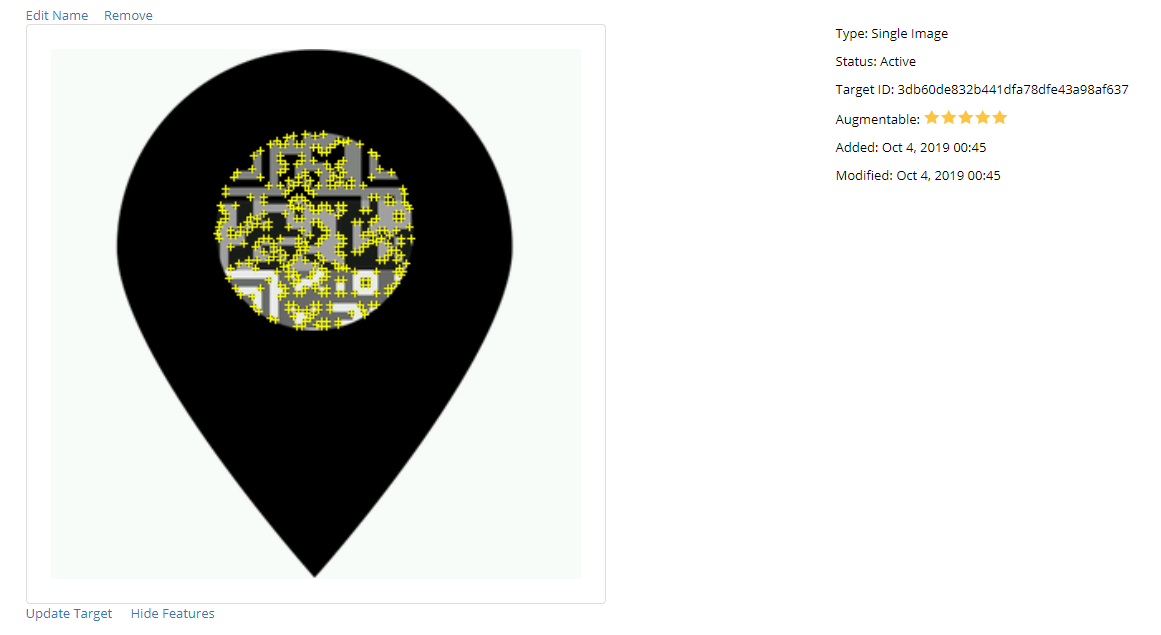
\includegraphics[width=14cm]{image_target_rating.PNG}
\caption{Image Target mit verwendeten Merkmalen und Rating}
\label{fig:image_target_rating}
\end{figure}

Beim Ausführen der Applikation wird von der Vuforia Engine eine Mustererkennung durchgeführt und die Kamerainformationen des Gerätes werden mit den Image-Target-Dateien verglichen. 
Im Falle einer Übereinstimmung wird eine zweite Mustererkennung gestartet, die den Abstand und die Rotation des Image Targets, mit dem erkannten Muster vergleicht.
Diese Informationen verwendet die Vuforia Engine dann, um die Größe und Ausrichtung des darzustellenden 3D Modells entsprechend anzupassen. (vgl. \cite{Grahn2017})
\section{Aufbau einer Unity-Applikation}\label{aufbau_unity_app}
Bevor in Abschnitt \ref{ch:realisierung_der_anwendung} näher auf die Nutzung von Unity für das gegebene IT Projekt eingegangen wird, wird im Folgenden der allgemeine Aufbau einer Unity-Anwendung erläutert. 

Unity ist, wie in Abschnitt \ref{entwicklungsumgebung} bereits kurz beschrieben, eine C++-basierte Spiele-Engine zum Entwerfen von Apps und Spielen, die plattformübergreifend exportiert werden können.

Ein Spiel besteht aus einer Zusammensetzung von Szenen, in welchen verschiedene Elemente, sogenannte \textquote{GameObjects}, hierarchisch in einem Szenengraph angeordnet sind. 
Ein GameObject ist die Basisklasse für alle Objekte in der Unity-Szene und hat standardmäßig keine visuellen Eigenschaften sondern nur einen Namen, ein Tag, eine Ebene und eine Transformation, welche die Position des Objekts im Raum beschreibt.
Dieses beschriebene leere GameObject ist mit seinen Standardeigenschaften in der rechten Leiste in Abbildung \ref{fig:gameObject_unity} dargestellt.
Bei Objekten, die in einer Eltern-Kind-Beziehung stehen, vererben Objekte in höheren Ebene ihre Position und Orientierungsinformationen an darunterliegende „Kind“-Objekte.

\begin{figure} [h]
\centering
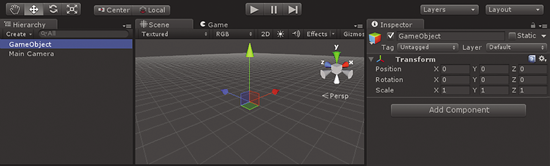
\includegraphics[width=15cm]{gameObject_unity.PNG}
\caption{leeres GameObject in Unity \cite{Tuplier2014}}
\label{fig:gameObject_unity}
\end{figure}

Da die GameObjects standardmäßig kein Aussehen und Verhalten haben, werden diese über sogenannte Komponenten, die einem GameObject angefügt werden können, definiert.
Diese stellen verschiedene Funktionen bereit, um das Verhalten und Aussehen der GameObjects zu bestimmen. 
Und werden unterteilt in vordefinierte Komponenten und dem speziellen Komponententyp \textquote{Script}.

Diese Scriptkomponente ist ebenfalls ein GameObject und ermöglicht es dem Benutzer, dem GameObject ein eigens definiertes Verhalten hinzuzufügen. 
Sie unterstützt die Programmierung in C\# und der an JavaScript angelehnten Programmiersprache UnityScript (vgl. \cite{Geiger2014}).

Abbildung \ref{fig:gameObject_unity_komponenten}. zeigt ein GameObject, dem mithilfe von Komponenten verschiedene visuelle Eigenschaften zugefügt wurden. Die Komponenten sind in der rechten Leiste des Editorfensters erkennbar.

\begin{figure} [h]
\centering
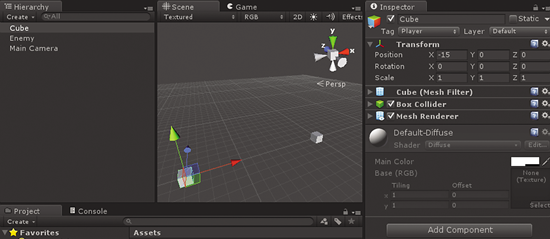
\includegraphics[width=15cm]{gameObject_unity_komponenten.PNG}
\caption{GameObject mit Komponenten \cite{Tuplier2014}}
\label{fig:gameObject_unity_komponenten}
\end{figure}

Alle beschriebenen Elemente sind in den Assets des Projektes zusammengefasst, welcher der oberste Ordner in der Unity-Ebene ist, in dem auch alle Medieninhalte hinterlegt sind.

Für die Implementierung von Augmented Reality Anwendungen ist ein Vuforia SDK für Unity verfügbar, welches verschiedene GameObjects zur Umsetzung von AR-Anwendungen enthält. Auf einige dieser wird im nachfolgenden Abschnitt \ref{einbindung_mustererkennung} eingegangen.